\label{sec:equations}
\section{Equations}
An equation is a statement that two mathematical expressions are equal. For example,
\begin{equation}
    2x + 3 = 5
\end{equation}

the letter $x$ is the variable. We think of $x$ as the “unknown” in the equation, and our goal
is to find the value of $x$ that makes the equation true. The values of the unknown that
make the equation true are called the \textbf{solutions} or \textbf{roots} of the equation, and the process
of finding the solutions is called \textbf{solving the equation}. \\

Two equations with exactly the same solutions are called \textbf{equivalent equations}. To
solve an equation, we try to find a simpler, equivalent equation in which the variable
stands alone on one side of the “equal” sign. Here are the properties that we use to solve
an equation. (In these properties, $A$, $B$, and $C$ stand for any algebraic expressions, and
the symbol 3 means “is equivalent to.”)

\begin{align*}
    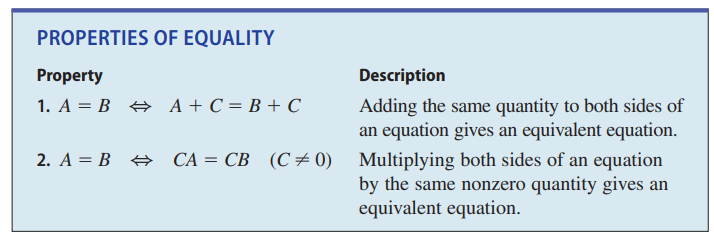
\includegraphics[width=1.1\textwidth]{algebra-pre-calculus/equations/properties_of_equations.png}
\end{align*}


\subsection{Solving Quadratic Equations}
\label{sec:quadratic-equations}
A quadratic equation is an equation that's highest exponent/power is 2. It can be written in the form of $ax^2+bx+c=0$ where $a,b,c$ are constants representing real numbers and $a \neq 0$. In this section we will go over how to solve quadratic equations.

\subsection{Solving quadratic equations by factoring}
For example: 
$$ 3x^2+7x-2=0$$ where $a=3$, $b=7$, and $c=-2$.
This also a quadratic equation but not in standard form: 
$$ 3x^2=-7x+2$$

The key to solve quadratic equations is: 
\begin{enumerate}
    \item Write it in standard form.
    \item Factor it or use the quadratic formula.
\end{enumerate}

\textbf{Example}. Find all real solutions for the equation $y^2=18-7y$
First following the steps is to re-write the equation in standard form.
$$y^2+7y-18=0$$
Then as we previously discussed during factoring we need to look for two numbers that multiply to $-18$ and add to $7$. The numbers are $9$ and $-2$.

Therefore, the equation can be factored as:
$$(y+9)(y-2)=0$$
Now for the equation to be true, one of the factors must be equal to zero. Therefore, $y+9=0$ or $y-2=0$. Solving for $y$ we get $y=-9$ or $y=2$. Therefore, the solutions for the equation are $y=-9$ or $y=2$.

You can check whether they are correct by substituting the values of $y$ in the original equation. So:
$$(-9)^2=18-7(-9)$$
$$81=18+63$$ which is true. Therefore, $y=-9$ is a solution.
To check for $y=2$:
$$(2)^2=18-7(2)$$
$$4=18-14$$ which is also true. Therefore, $y=2$ is also a solution.
\newpage
\textbf{Example}. Solve the equation $w^2=121$ \\
First we need to re-write the equation in standard form:
$$w^2-121=0$$ where $a=1$, $b=0$, and $c=-121$.
Then we need to factor the equation. We can factor it as:
$$(w+11)(w-11)=0$$ Because $w^2-121=(w+11)(w-11)$. \\

Again, for the equation to be true, one of the factors must be equal to zero. Therefore, $w+11=0$ or $w-11=0$. Solving for $w$ we get $w=-11$ or $w=11$. Therefore, the solutions for the equation are $w=-11$ or $w=11$.

Now we could have solved the equation by taking the square root of both sides. So:
\begin{align*}
    w^2&=121 \\
    \sqrt{w^2}&=\pm \sqrt{121} \\
    w&=\pm 11
\end{align*}

The reason why we have to take plus and minus is because when we take the square root of both sides we get $w=\pm 11$ because $11^2=121$ and $(-11)^2=121$ as well.

\textbf{Example}. Solve the equation $x(x+2) = 7$
\\
First we need to re-write the equation in standard form by multiplying out and subtracting $7$ from both sides:
$$x^2+2x-7=0$$ where $a=1$, $b=2$, and $c=-7$.
Now again we are looking for two numbers that multiply to $-7$ and add to $2$. Unfortunately, there are no two whole numbers that multiply to $-7$ and add to $2$. Therefore, we can't factor the equation. So we have to use the quadratic formula to solve the equation.
\subsection{Quadratic formula}
The quadratic formula is a formula that gives the solutions for a quadratic equation. In our example $a = 1$, $b = 2$, and $c = -7$. So the quadratic formula is:
$$x=\frac{-b \pm \sqrt{b^2-4ac}}{2a}$$
So plugging in the values of $a$, $b$, and $c$ we get:
$$x=\frac{-2 \pm \sqrt{2^2-4(1)(-7)}}{2(1)}$$

Simplifying we get:
$$x=\frac{-2 \pm \sqrt{32}}{2} = \frac{-2\pm\sqrt{16\cdot2}}{2} = \frac{-2\pm4\sqrt{2}}{2} $$
Simplifying everything we get: 
$$ -1\pm2\sqrt{2} $$
So the solutions are: $x=-1+2\sqrt{2}$ or $x=-1-2\sqrt{2}$.

\textbf{Example}. Solve the equation $\frac{1}{2}y^2 = \frac{1}{3}y-2$ \\

First we need to re-write the equation in standard form by multiplying out and subtracting $\frac{1}{3}y-2$ from both sides:
$$\frac{1}{2}y^2-\frac{1}{3}y+2=0$$ where $a=\frac{1}{2}$, $b=-\frac{1}{3}$, and $c=2$.

Let's get rid of the denominator by multiplying both sides by $6$ which is the least common multiple of $2$ and $3$:
$$3y^2-2y+12=0$$ where $a=3$, $b=-2$, and $c=12$.

Now let's use the quadratic formula to solve the equation:
$$x=\frac{2\pm\sqrt{(-2)^2-4(3)(12)}}{2(3)}$$

Simplifying we get:
$$x=\frac{2\pm\sqrt{4-144}}{6} = \frac{2\pm\sqrt{-140}}{6}$$

Since we cannot square negative numbers this equation has no real solutions. 
The reason why we cannot square negative numbers is because any number squared will produce a positive number, so there is no true square root of a negative number.

The steps to solve quadratic equations are:
\begin{enumerate}
    \item Write the equation in standard form.
    \item Factor the equation or use the quadratic formula. Because factoring is not always possible, but the quadratic formula always works. Therefore, you can't really lose by using the quadratic formula, however sometimes it is easier and faster to factor the equation.
\end{enumerate}

The quantity $b^2-4ac$ is called the \textbf{discriminant} of the quadratic equation $ax^2+bx+c=0$ and is denoted by the symbol $D$. If $D>0$, then the equation has two real solutions. If $D=0$, then the equation has one real solution. If $D<0$, then the equation has no real solutions. 

\begin{align*}
    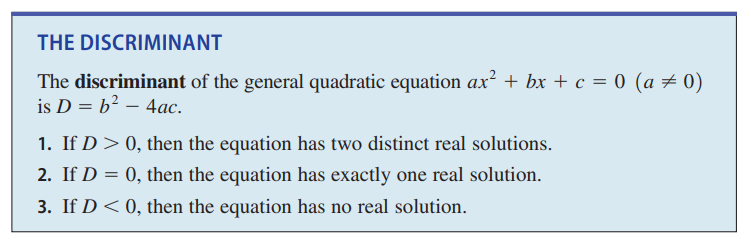
\includegraphics[width=1.1\textwidth]{algebra-pre-calculus/equations/discriminant.png}
\end{align*}

\subsection{Solving quadratic equations by completing the square}
If a quadratic equation does not factor readily, then we can solve it using the technique of \textbf{completing the square}.
This means that we add a constant to an expression to make it a perfect square. For example, to make $x^2-6x$ a perfect square, we must add $9$, since $(x-3)^2=x^2-6x+9$. \\
Being aware of the standard form: $ax^2+bx+c=0$:

\begin{align*}
    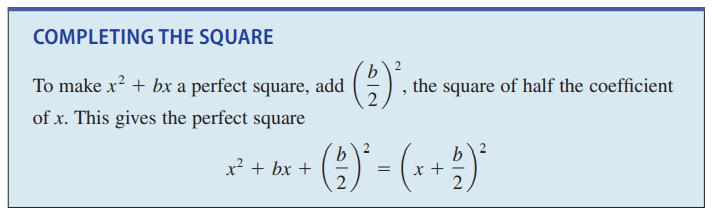
\includegraphics[width=1.1\textwidth]{algebra-pre-calculus/equations/completing_square.png}
\end{align*}

\textbf{(a)} $x^2-8x+13=0$

\begin{align*}
    x^2-8x+13&=0 \\
    x^2-8x&=-13 \quad  \color{blue}\text{Subtract 13} \\ 
    x^2-8x+\color{blue}{16}&=-13+\color{blue}{16} \quad \color{blue}\text{Complete the square: add} \ \left(\frac{-8}{2}\right)^2\\
    (x-4)^2&=3 \quad  \color{blue}\text{Perfect square} \\
    x-4&=\pm\sqrt{3} \quad  \color{blue}\text{Take square root} \\
    x&=4\pm\sqrt{3} \quad  \color{blue}\text{Add 4}
\end{align*}

\textbf{(b)} $3x^2-12x+6=0$

\begin{align*}
    3x^2-12x+6&=0 \\
    3x^2-12x&=-6 \quad  \color{blue}\text{Subtract 6} \\ 
    3(x^2-4x)&=-6 \quad \color{blue}\text{Factor 3}\\
\end{align*}
Now we complete the square by adding $\displaystyle\left(\frac{-4}{2}\right)^2=4$ \textbf{inside the parentheses}. Since everything inside the parentheses is multiplied by 3, this means that we are actually adding $3\cdot4=12$ to the left side of the equation. Therefore, we must also add $12$ to the right side of the equation to keep it equal.

\begin{align*}
    3(x^2-4x+4)&=-6+12 \quad \color{blue}\text{Complete the square: add} \ 4 \\
    3(x-2)^2&=6 \quad  \color{blue}\text{Perfect square} \\
    (x-2)^2&=2 \quad  \color{blue}\text{Divide by 3} \\
    x-2&=\pm\sqrt{2} \quad  \color{blue}\text{Take square root} \\
    x&=2\pm\sqrt{2} \quad  \color{blue}\text{Add 2}
\end{align*}

\subsection{Solving A Fourth-Degree Equation of Quadratic Type}
An equation of the form $aW^2+bW+c=0$, where $W$ is an algebraic expression,
is an equation of \textbf{quadratic type.} We solve equations of quadratic type by substituting
for the algebraic expression, as we see in the next two examples. 

\textbf{(a)} Find all real solutions of the equation $x^4-8x^2+8=0$.

If we go ahead and set the $W$ variable to $x^2$, we get the equation $W^2-8W+8=0$.

In other words, in our equation we can solve it as so,


\begin{align*}
   &(x^2)^2-8x^2+8=0 \quad \color{blue}\text{Write} \ x^4 \text{as} (x^2)^2 \\
   &W^2-8W+8=0 \quad \color{blue}\text{Substitute} \ W=x^2 \\
   &W=\frac{8\pm\sqrt{(-8)^2-4(1)(8)}}{2(1)} \quad \color{blue}\text{Use the quadratic formula} \\
   &x^2=4\pm2\sqrt{2} \quad \color{blue}W=x^2 \\
   &x=\pm\sqrt{4\pm2\sqrt{2}} \quad \color{blue}\text{Take square root} \\
\end{align*}

So there are four solutions: $x=\sqrt{4+2\sqrt{2}}$, $x=-\sqrt{4+2\sqrt{2}}$, $x=\sqrt{4-2\sqrt{2}}$, and $x=-\sqrt{4-2\sqrt{2}}$.

\subsection{Fractional Power Equations - Quadratic Type}

Find all solutions of the equation $x^{\frac{1}{3}}+x^{\frac{1}{6}}-2=0$

This equation is of quadratic type because if we let $W=x^{\frac{1}{6}}$, then
$W^2=x^{\frac{1}{3}}$. So we can solve the equation as so,

\begin{align*}
    &W^2 + W - 2 = 0 \quad \text{\color{blue} Substitute } W = x^{1/6} \\
    &(W - 1)(W + 2) = 0 \quad \text{\color{blue} Factor} \\
    &\begin{aligned}
        W - 1 &= 0 \hspace{2cm}  W + 2= 0 \\
        W &= 1 \hspace{2cm}  W= -2 \\
        x^{1/6} &= 1 \hspace{2cm}  x^{1/6}= -2 \\	
        x &= 1^6 \hspace{2cm}  x= (-2)^6 \\
        x &= 1 \hspace{2cm}  x= 64 \\
    \end{aligned}
\end{align*}

From \textbf{Check Your Answers} we see that $x=1$ is a solution but $x=64$ is not. The only
solution is $x=1$.